% !TeX spellcheck = en_US
% !TeX encoding = utf8
% !TeX program = xelatex
% !BIB program = bibtex

% \documentclass[mathserif,compress,12pt]{ctexbeamer}
\documentclass[12pt,notes,mathserif]{beamer}
% \documentclass[draft]{beamer}	
\usetheme{Singapore}
% \usetheme{Hannover}
%\usepackage{pgfpages}
%\setbeameroption{show notes on second screen}

\usepackage[british]{babel}
\usepackage{graphicx,hyperref,url}
% \usepackage{ru}
\usepackage{mmstyles}

\usepackage{listings}
\usefonttheme[onlymath]{serif}
\usepackage{fontspec}
\usepackage{xeCJK}
% \pgfdeclareimage[width=\paperwidth,height=\paperheight]{bg}{background}
% \setbeamertemplate{background}{\pgfuseimage{bg}}
%% columns
\newcommand{\begincols}[1]{\begin{columns}{#1}}
\newcommand{\stopcols}{\end{columns}}
% \usepackage[backend=biber]{biblatex}
% \bibliography{./ref.bib}
%\addbibresource{ref.bib}
\usepackage{indentfirst}
\usepackage{longtable}
\usepackage{float}
%\usepackage{picins}
\usepackage{rotating}
\usepackage{subfigure}
\usepackage{tabu}
\usepackage{amsmath}
\usepackage{amssymb}
\usepackage{setspace}
\usepackage{amsfonts}
\usepackage{appendix}
\usepackage{listings}
\usepackage{xcolor}
\usepackage{colortbl}
\usepackage{geometry}
% \setCJKfamilyfont{cjkhwxk}{SimSun}
% \newcommand*{\cjkhwxk}{\CJKfamily{cjkhwxk}}
%\newfontfamily{\consolas}{Consolas}
%\newfontfamily{\monaco}{Monaco}
%\setmonofont[Mapping={}]{Consolas}	%英文引号之类的正常显示,相当于设置英文字体
%\setsansfont{Consolas} %设置英文字体 Monaco, Consolas,  Fantasque Sans Mono
% \setmainfont{Times New Roman}
% \newfontfamily{\consolas}{Times New Roman}
% \newfontfamily{\monaco}{Arial}
% \setCJKmainfont{Times New Roman}
%\setmainfont{MONACO.TTF}
%\setsansfont{MONACO.TTF}
\newcommand{\verylarge}{\fontsize{60pt}{\baselineskip}\selectfont}  
\newcommand{\chuhao}{\fontsize{44.9pt}{\baselineskip}\selectfont}  
\newcommand{\xiaochu}{\fontsize{38.5pt}{\baselineskip}\selectfont}  
\newcommand{\yihao}{\fontsize{27.8pt}{\baselineskip}\selectfont}  
\newcommand{\xiaoyi}{\fontsize{25.7pt}{\baselineskip}\selectfont}  
\newcommand{\erhao}{\fontsize{23.5pt}{\baselineskip}\selectfont}  
\newcommand{\xiaoerhao}{\fontsize{19.3pt}{\baselineskip}\selectfont} 
\newcommand{\sihao}{\fontsize{14pt}{\baselineskip}\selectfont}      % 字号设置  
\newcommand{\xiaosihao}{\fontsize{12pt}{\baselineskip}\selectfont}  % 字号设置  
\newcommand{\wuhao}{\fontsize{10.5pt}{\baselineskip}\selectfont}    % 字号设置  
\newcommand{\xiaowuhao}{\fontsize{9pt}{\baselineskip}\selectfont}   % 字号设置  
\newcommand{\liuhao}{\fontsize{7.875pt}{\baselineskip}\selectfont}  % 字号设置  
\newcommand{\qihao}{\fontsize{5.25pt}{\baselineskip}\selectfont}    % 字号设置 

\graphicspath{{./fig/}}

% \setbeamertemplate{footnote}{%
%   \hangpara{2em}{1}%
%   \makebox[2em][l]{\insertfootnotemark}\footnotesize\insertfootnotetext\par%
% }

\definecolor{cred}{rgb}{0.6,0,0}
\definecolor{cgreen}{rgb}{0.25,0.5,0.35}
\definecolor{cpurple}{rgb}{0.5,0,0.35}
\definecolor{cdocblue}{rgb}{0.25,0.35,0.75}
\definecolor{cdark}{rgb}{0.95,1.0,1.0}
\lstset{
	language=R,
	numbers=left,
	numberstyle=\tiny\color{black},
	keywordstyle=\color{cpurple}\consolas,
	commentstyle=\color{cgreen}\consolas,
	stringstyle=\color{cred}\consolas,
	frame=single,
	escapeinside=``,
	xleftmargin=1em,
	xrightmargin=1em, 
	backgroundcolor=\color{cdark},
	aboveskip=1em,
	breaklines=true,
	tabsize=3
} 

\providecommand{\tightlist}{%
  \setlength{\itemsep}{0pt}\setlength{\parskip}{0pt}}

  
% The title of the presentation:
%  - first a short version which is visible at the bottom of each slide;
%  - second the full title shown on the title slide;
% \title[]{\LARGE CSE 5526: Introduction to Neural Networks}

% Optional: a subtitle to be dispalyed on the title slide
\title{Radial Basis Function (RBF) Networks}

% The author(s) of the presentation:
%  - again first a short version to be displayed at the bottom;
%  - next the full list of authors, which may include contact information;
\author[YingmingLi]{Yingming Li \\ yingming@zju.edu.cn}
% The institute:
%  - to start the name of the university as displayed on the top of each slide
%    this can be adjusted such that you can also create a Dutch version
%  - next the institute information as displayed on the title slide

\institute[DSERC, ZJU]{Data Science \& Engineering Research Center, ZJU}
% Add a date and possibly the name of the event to the slides
%  - again first a short version to be shown at the bottom of each slide
%  - second the full date and event name for the title slide
\date[\today]{\today}

\begin{document}

\AtBeginSection[]
{
	\begin{frame}
		\frametitle{Outline}
		\tableofcontents[currentsection]
	\end{frame}
}

% \AtBeginSubsection[2-]
% {
%    \begin{frame}
%        \frametitle{Outline}
%        \tableofcontents[currentsection]
%    \end{frame}
% }
\begin{frame}[c]
	\titlepage
	\begin{center}
		Adapted from slides provided by Prof.  Michael Mandel.
	\end{center}
\end{frame}

% 2
\begin{frame}[c]
	\frametitle{Function approximation}
	\begin{itemize}
		\item We have been using MLPs as pattern classifiers
		\item But in general, they are function approximators
		      \begin{itemize}
			      \item Depending on output layer nonlinearity
			      \item And error function being minimized
		      \end{itemize}
		\item As a function approximator, MLPs are nonlinear, semiparametric, and universal
	\end{itemize}
\end{frame}
% 3
\begin{frame}[c]
	\frametitle{Function approximation}
	\begin{itemize}
		\item  Radial basis function (RBF) networks are similar function approximators
		\item Also nonlinear, semiparametric, universal
		\item Can also be visualized as layered network of nodes
		\item Easier to train than MLPs
		      \begin{itemize}
			      \item Do not require backpropagation
			      \item But do not necessarily find an optimal solution
		      \end{itemize}
	\end{itemize}
\end{frame}

% 4
\begin{frame}[c]
	\frametitle{RBF net illustration}
	\begin{center}
		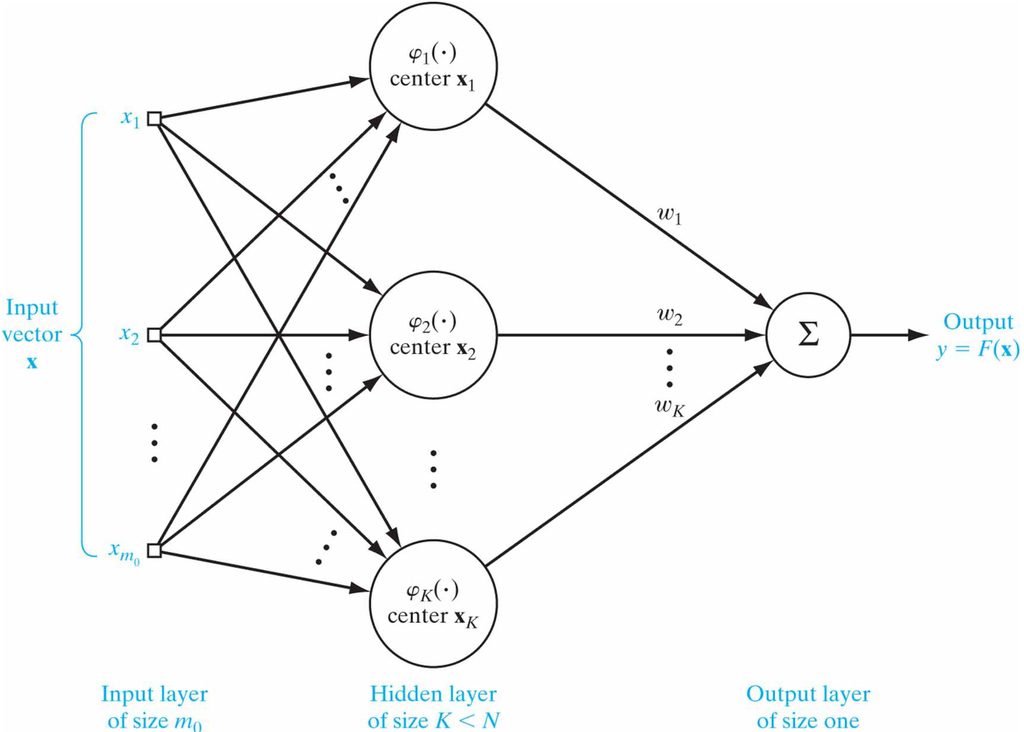
\includegraphics[width=0.9\linewidth]{fig/lec74.jpg}
	\end{center}
\end{frame}
% 5
\begin{frame}[c]
	\frametitle{Function approximation background}
	\begin{itemize}
		\item Before getting into RBF networks, let's discuss approximating scalar functions of a single variable
		\item Weierstrass approximation theorem: any continuous real function in an interval can be approximated arbitrarily well by a set of polynomials

		\item  Taylor expansion approximates any differentiable function by a polynomial in the neighborhood around a point

		\item  Fourier series gives a way of approximating any periodic function by a sum of sines and cosines
	\end{itemize}
\end{frame}

% 6
\begin{frame}[c]
	\frametitle{Linear projection}
	\begin{itemize}
		\item Approximate function $f(x)$ by a linear combination of simpler functions
		      \[
			      f(\mathbf{x})=\sum_jw_j\varphi_j(\mathbf{x})
		      \]
		\item If $w_j$'s can be chosen so that approximation error is arbitrarily small for any function $f(x)$ over the domain of interest, then $\{\varphi_j\}$ has the property of universal approximation, or $\{\varphi_j\}$ is complete𝑗

	\end{itemize}
\end{frame}
% 7
\begin{frame}[c]
	\frametitle{Example incomplete basis: $\mathrm{sinc}$}
	\[
		\mathrm{sinc}(x)=\frac{\sin(\pi x)}{\pi x}\qquad
		\varphi_j(x)=\mathrm{sinc}(x-\mu_j)
	\]\vspace*{-5mm}
	\begin{itemize}
		\item Can approximate any smooth function
	\end{itemize}
	\begin{figure}
		\centering
		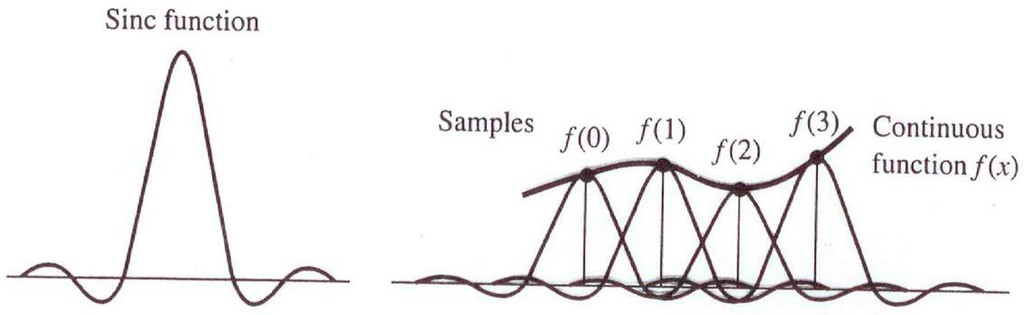
\includegraphics[width=0.85\linewidth]{fig/lec77.jpg}
		\caption{Decomposition by sinc functions}
	\end{figure}
\end{frame}

% 8
\begin{frame}[c]
	\frametitle{Example orthogonal complete basis: sinusoids}
	\begin{equation*}
		\begin{array}{c}
			\varphi_{2n}(x)=\sin (2\pi n\omega x)   \\[2mm]
			\varphi_{2n+1}(x)=\cos (2\pi n\omega x) \\[2mm]
			{\rm Complete~on~the~interval}~[0,1]
		\end{array}
	\end{equation*}
	\begin{figure}
		\centering
		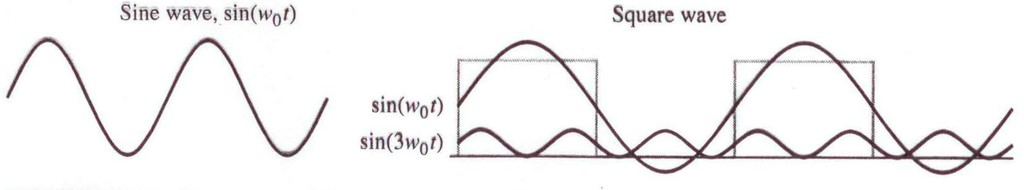
\includegraphics[width=0.95\linewidth]{fig/lec78.jpg}
		\caption{Decomposition by sine waves}
	\end{figure}
\end{frame}

% 9
\begin{frame}[c]
	\frametitle{Example orthogonal complete basis: Chebyshev polynomials}
	\begin{equation*}
		\begin{array}{c}
			T_0(x)=1\qquad
			T_1(x)=1\qquad
			T_{n+1}(x)=2xT_n(x)-T_{n-1}(x)       \\[2mm]
			{\rm Complete~on~the~interval}~[0,1] \\[2mm]
			T_2(x)=2x^2-1\qquad
			T_3(x)=4x^3-3x\quad {\rm etc.}
		\end{array}
	\end{equation*}
	\begin{center}
		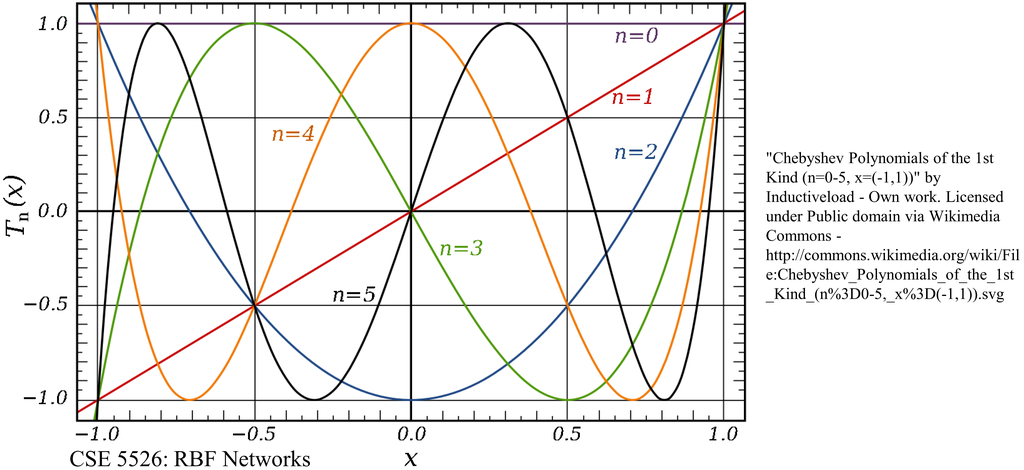
\includegraphics[width=0.85\linewidth]{fig/lec79.jpg}
	\end{center}
\end{frame}

% 10
\begin{frame}[c]
	\frametitle{Radial basis functions}
	\begin{itemize}
		\item 𝑖A radial basis function (RBF) is a basis function of the form $\varphi_j(\mathbf{x})=\varphi(||\mathbf{x}-\vmu_j||)$

		      \begin{itemize}
			      \item Where $\varphi(r)$ should be positive with monotonic derivative for $r> 0$. 
		      \end{itemize}
		\item Consider a Gaussian RBF
		      \[
			      \varphi_j(\mathbf{x})=\exp\left(-\dfrac{1}{2\sigma^2}||\mathbf{x}-\mathbf{x}_j||^2\right)=G(||\mathbf{x}-\mathbf{x}_j||)
		      \]
		\item A \textit{local} basis function, falling off from the center
		      \begin{center}
			      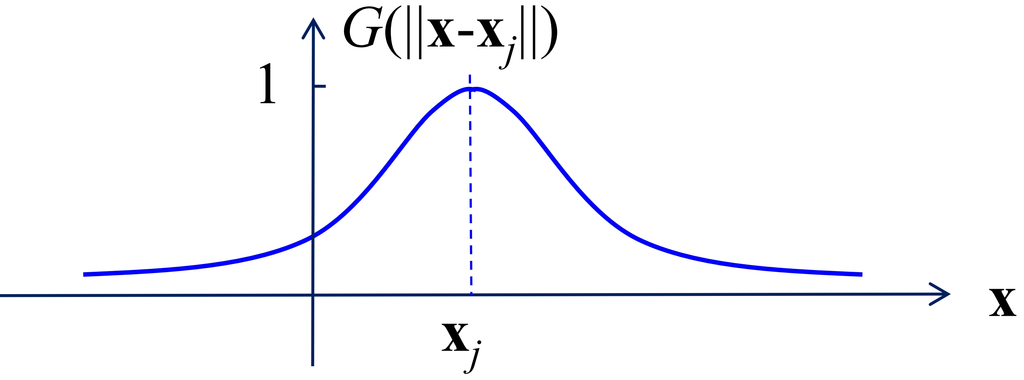
\includegraphics[width=0.85\linewidth]{fig/lec710.jpg}
		      \end{center}
	\end{itemize}
\end{frame}

% 11
\begin{frame}[c]
	\frametitle{Radial basis functions (cont.)}
	\begin{itemize}
		\item Thus approximation by Gaussian RBF becomes
		      \[
			      F(\mathbf{x})=\sum_jw_jG(||\mathbf{x}-\mathbf{x}_j||)
		      \]
		\item Gaussians are universal approximators
		      \begin{itemize}
			      \item \ie, they form a complete basis
		      \end{itemize}
	\end{itemize}
	\begin{center}
		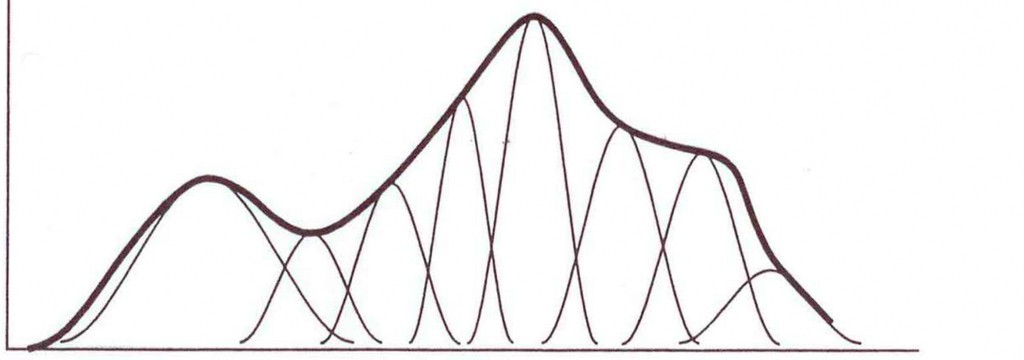
\includegraphics[width=0.99\linewidth]{fig/lec711.jpg}
	\end{center}
\end{frame}

% 12
\begin{frame}[c]
	\frametitle{RBF net illustration}
	\begin{figure}
		\centering
		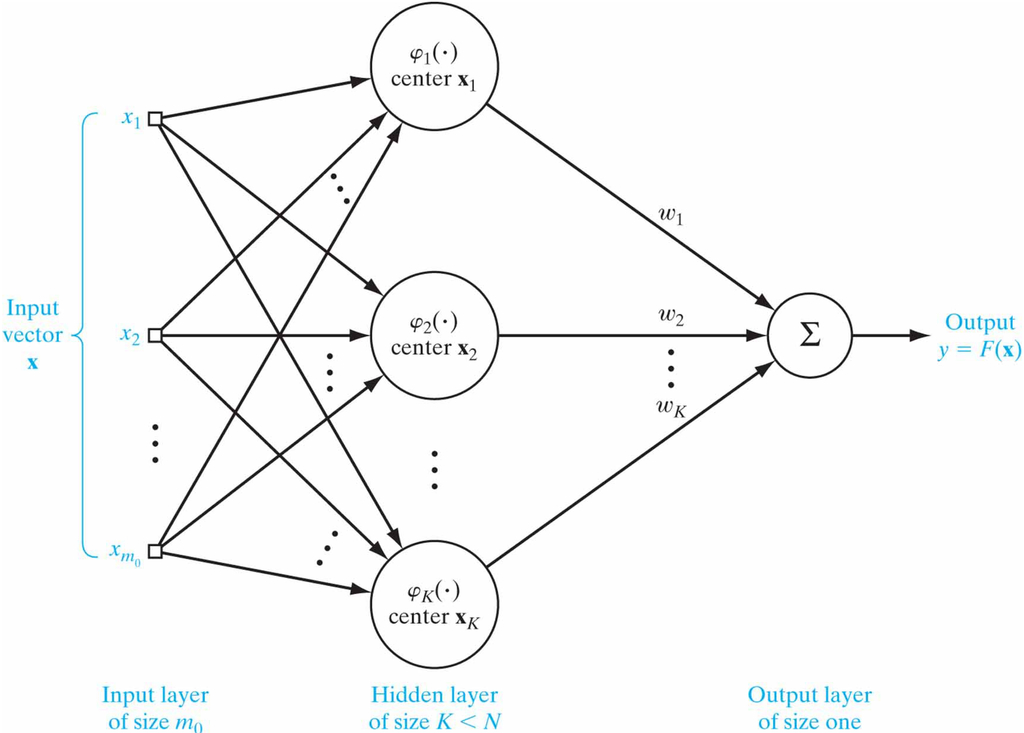
\includegraphics[width=0.99\linewidth]{fig/lec712.jpg}
		\caption{Approximation by RBFs in one dimension}
	\end{figure}
\end{frame}

% 13
\begin{frame}[c]
	\frametitle{Remarks (cont.)}
	\begin{itemize}
		\item Other RBFs exist, but we won't be using them
		\item Multiquadrics
		      \[
			      \varphi(x)=\sqrt{x^2+c^2}
		      \]
		\item Inverse multiquadrics
		      \[
			      \varphi(x)=\frac{1}{\sqrt{x^2+c^2}}
		      \]
		\item Micchelli's theorem (1986)
		      \begin{itemize}
			      \item Let $\{x_i\}$ be a set of $N$ distinct points, $\varphi(\cdot)$ be an RBF
			      \item Then the matrix $\phi_{ij}=\varphi(||\mathbf{x}_i-\mathbf{x}_j||)$ is non-singular
		      \end{itemize}
	\end{itemize}
\end{frame}

% 14
\begin{frame}[c]
	\frametitle{Four questions to answer for RBF nets}
	\begin{itemize}
		% \tightlist
		\item If we want to use Gaussian RBFs to approximate a function specified by training data
		      \begin{enumerate}
			    %   \tightlist
			      \item How do we choose the Gaussian centers?
			      \item How do we determine the Gaussian widths?
			      \item How do we determine the weights $w_j$?
			      \item How do we select the number of bases?
		      \end{enumerate}
	\end{itemize}
\end{frame}


% 15
\begin{frame}[c]
	\frametitle{1. How do we choose the Gaussian centers?}
	\begin{itemize}
		\tightlist
		\item Easy way: select K data points at random
		\item Potentially better way: unsupervised clustering, e.g. using the K-means algorithm
	\end{itemize}
\end{frame}

% 16
\begin{frame}[c]
	\frametitle{K-means algorithm}
	\begin{itemize}
		\item Goal: Divide $N$ input patterns into $K$ clusters with minimum total variance In other words, partition patterns into $K$ clusters 𝐶𝐶
		\item In other words, partition patterns into $K$ clusters $C_j$ to minimize the following cost function
		      \[
			      J=\sum_{j=1}^K\sum_{i\in C_j} ||\mathbf{x}_i-\mathbf{u}_j||^2
		      \]
		      where $\mathbf{u}_j=\dfrac{1}{|C_j|}\sum_{i\in C_j}\mathbf{x}_i$ is  the mean (center) of cluster~$j$
	\end{itemize}
\end{frame}

% 17
\begin{frame}[c]
	\frametitle{K-means algorithm}
	\begin{enumerate}
		\item Choose a set of $K$ cluster centers randomly from the input patterns
		\item Assign the $N$ input patterns to the $K$ clusters using the squared Euclidean distance rule:

		      $\vx$ is assigned to $C_j$ if $||\mathbf{x}-\mathbf{u}_j||^2\le ||\mathbf{x}-\mathbf{u}_i||^2$ for all $i\neq j$
		\item Update cluster centers
		      \[
			      \mathbf{u}_j=\frac{1}{|C_j|}\sum_{i\in C_j}\mathbf{x}_i
		      \]
		\item If any cluster center changes, go to step 2; else stop
	\end{enumerate}
\end{frame}



% 18
\begin{frame}[c]
	\frametitle{K-means illustration}
	\begin{center}
		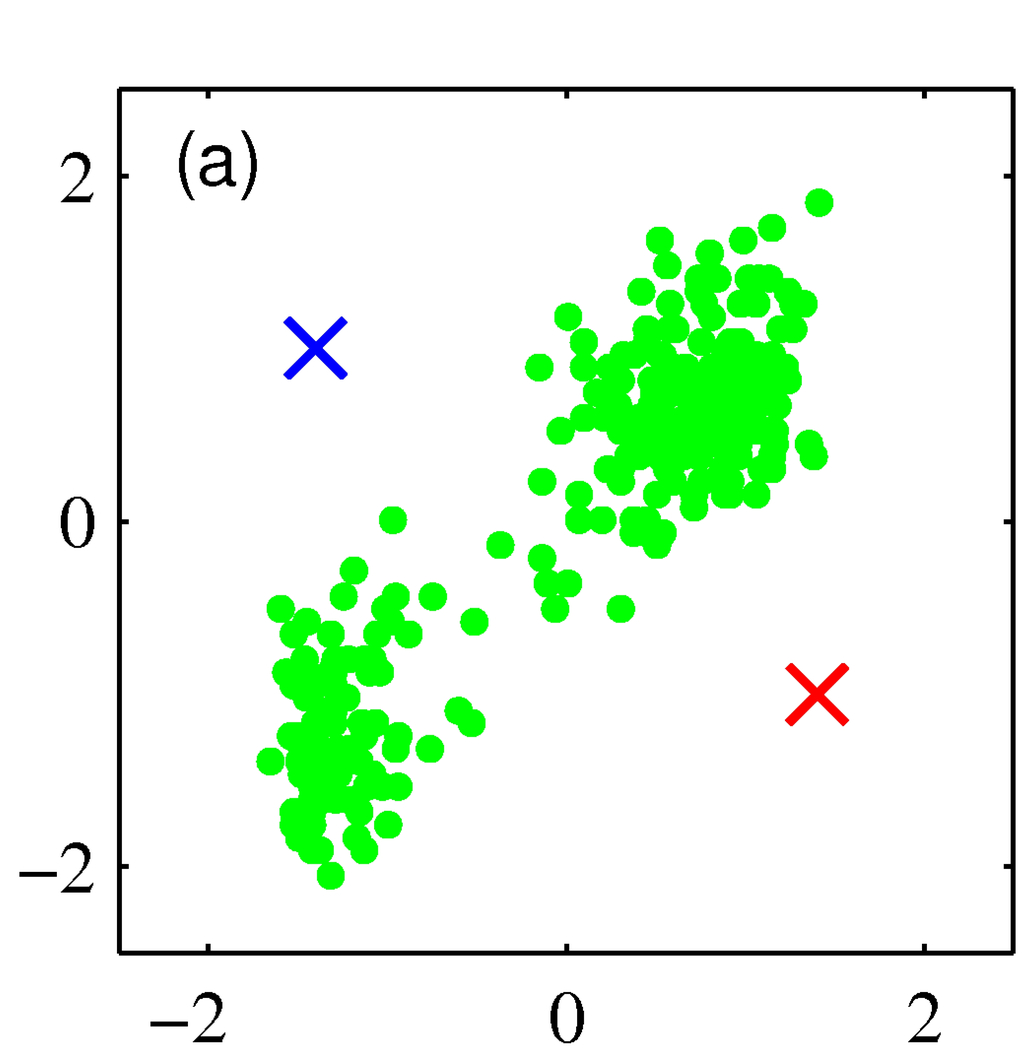
\includegraphics[width=0.65\textwidth]{fig/lec718.jpg}
	\end{center}
\end{frame}


% 19
\begin{frame}[c]
	\frametitle{K-means illustration}
	\begin{center}
		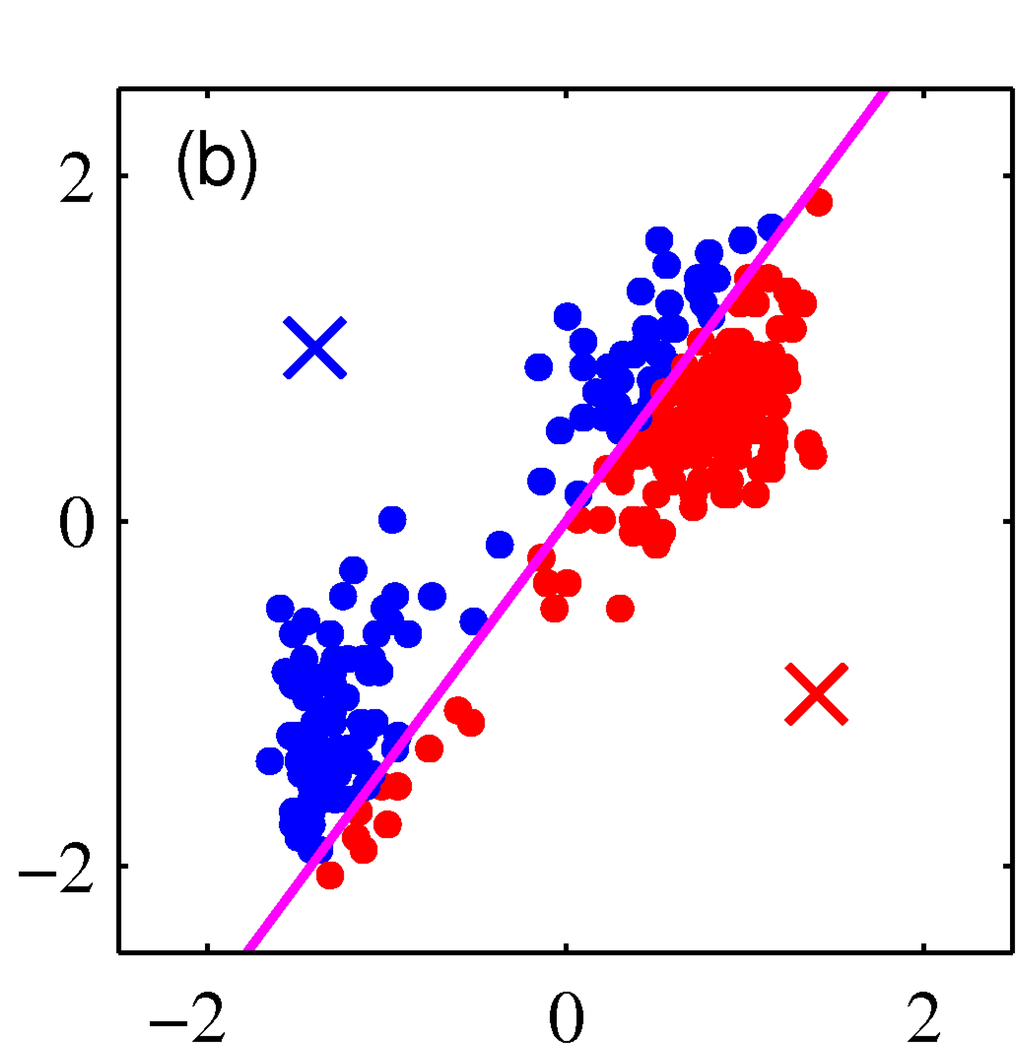
\includegraphics[width=0.65\textwidth]{fig/lec719.jpg}
	\end{center}
\end{frame}
% 20
\begin{frame}[c]
	\frametitle{K-means illustration}
	\begin{center}
		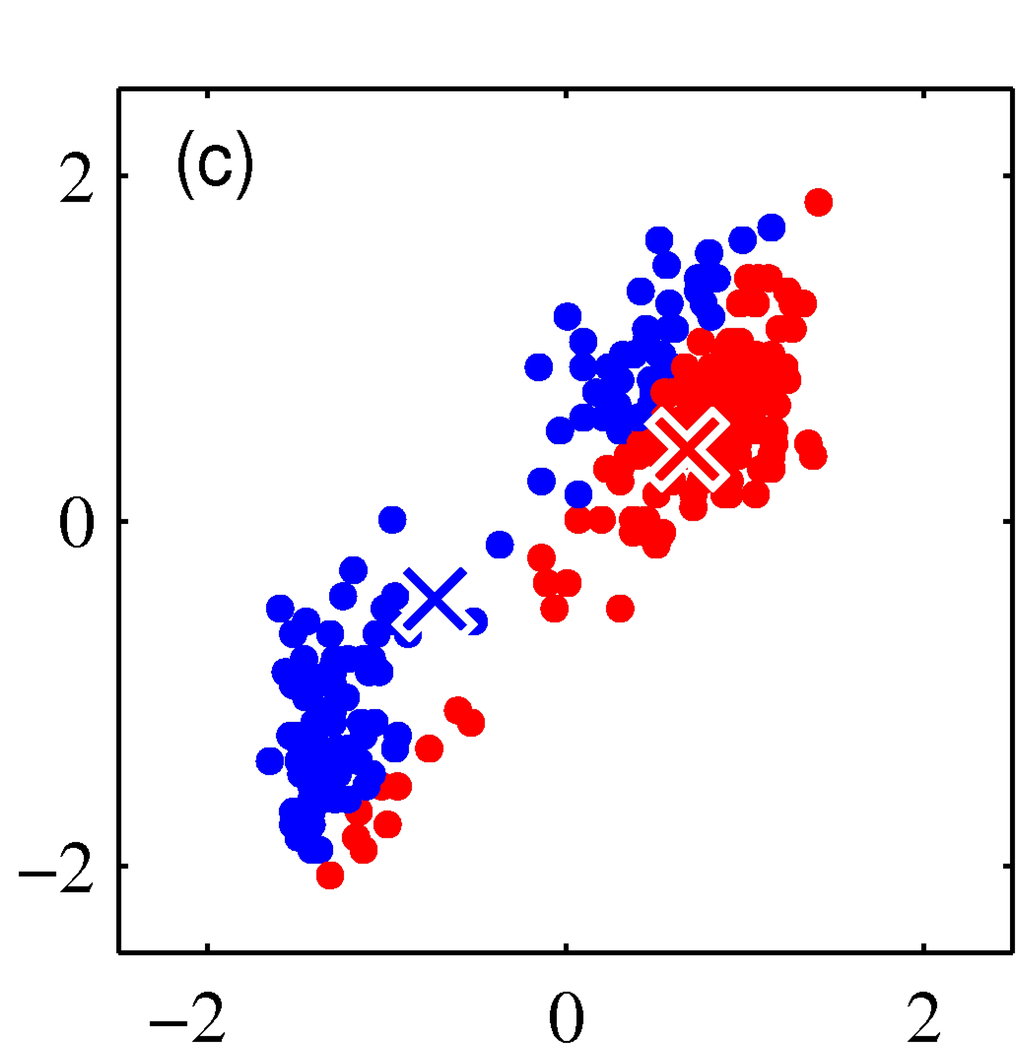
\includegraphics[width=0.65\textwidth]{fig/lec720.jpg}
	\end{center}
\end{frame}
% 21
\begin{frame}[c]
	\frametitle{K-means illustration}
	\begin{center}
		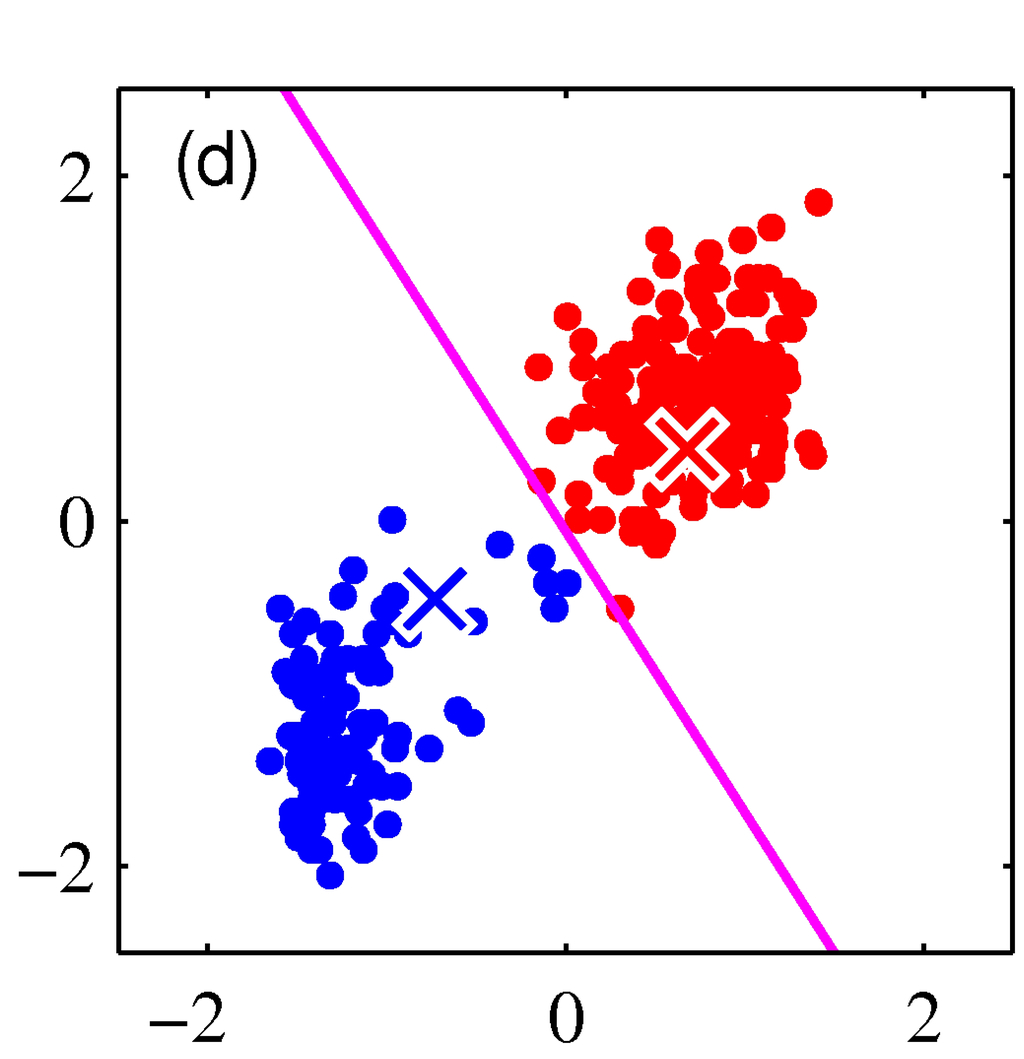
\includegraphics[width=0.65\textwidth]{fig/lec721.jpg}
	\end{center}
\end{frame}

% 22
\begin{frame}[c]
	\frametitle{K-means illustration}
	\begin{center}
		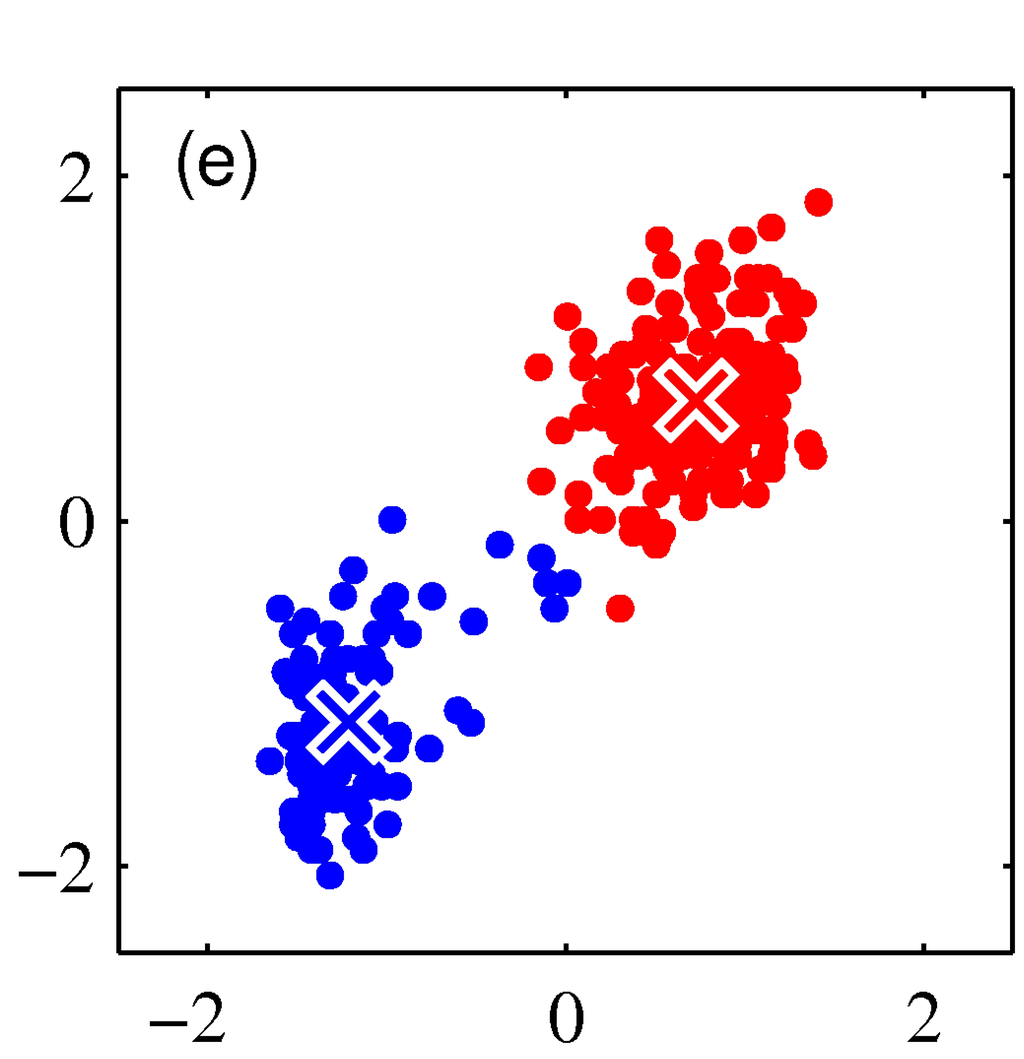
\includegraphics[width=0.65\textwidth]{fig/lec722.jpg}
	\end{center}
\end{frame}

% 23
\begin{frame}[c]
	\frametitle{K-means illustration}
	\begin{center}
		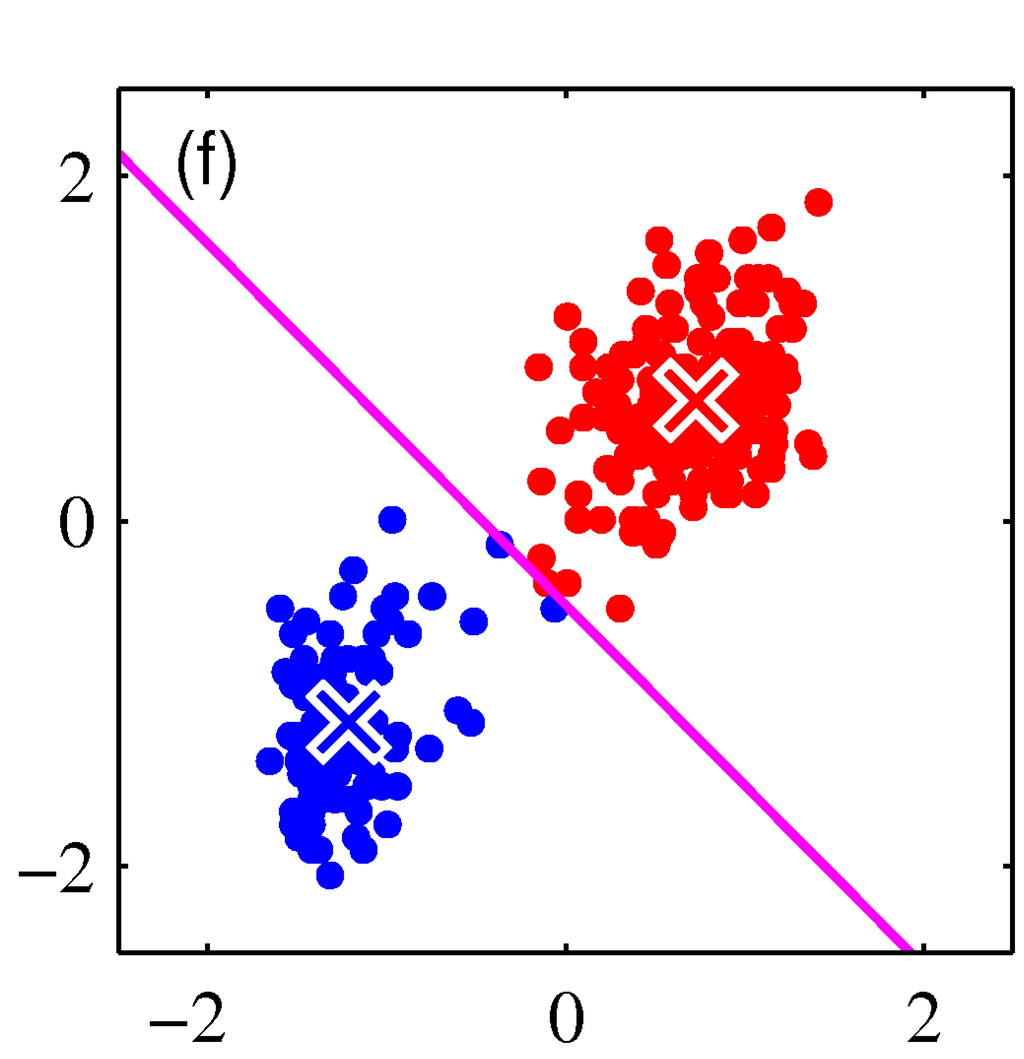
\includegraphics[width=0.65\textwidth]{fig/lec723.jpg}
	\end{center}
\end{frame}

% 24
\begin{frame}[c]
	\frametitle{K-means illustration}
	\begin{center}
		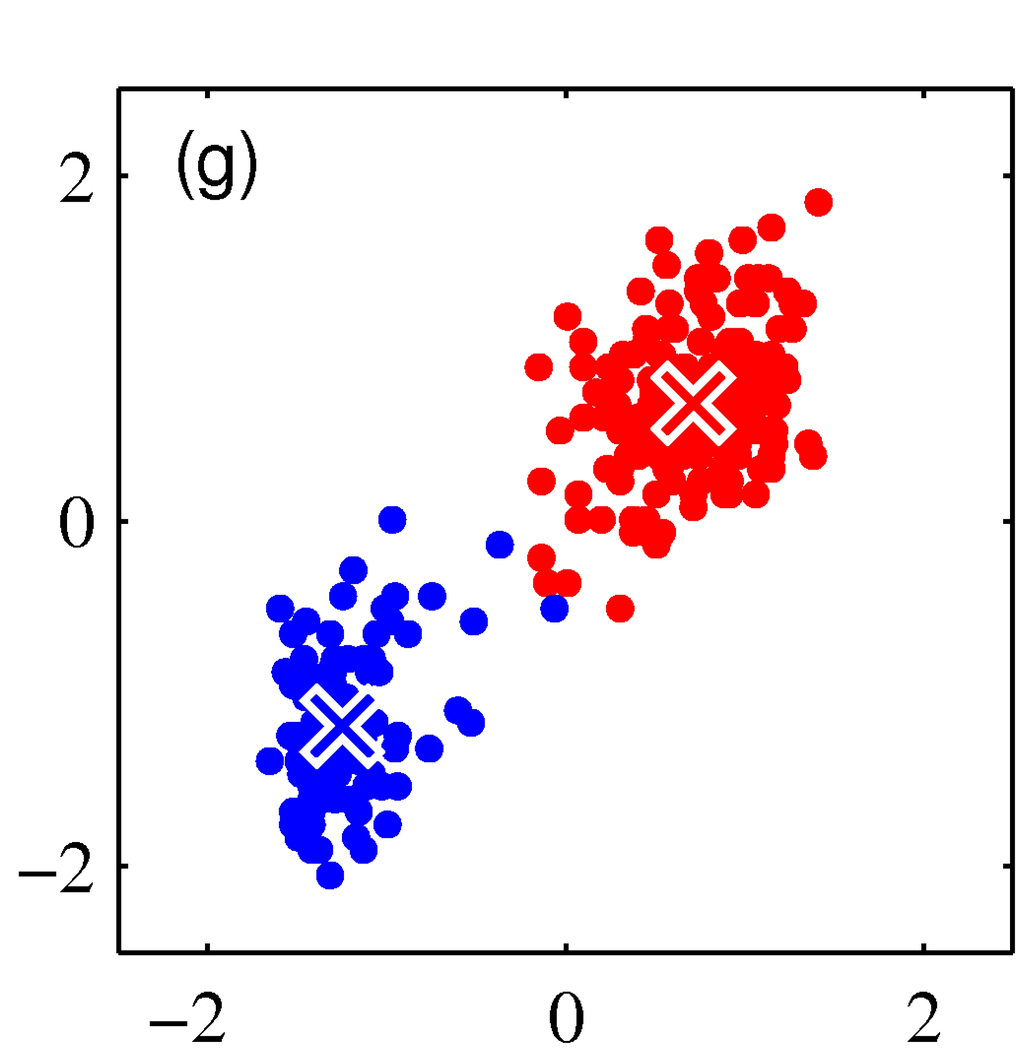
\includegraphics[width=0.65\textwidth]{fig/lec724.jpg}
	\end{center}
\end{frame}

% 25
\begin{frame}[c]
	\frametitle{K-means illustration}
	\begin{center}
		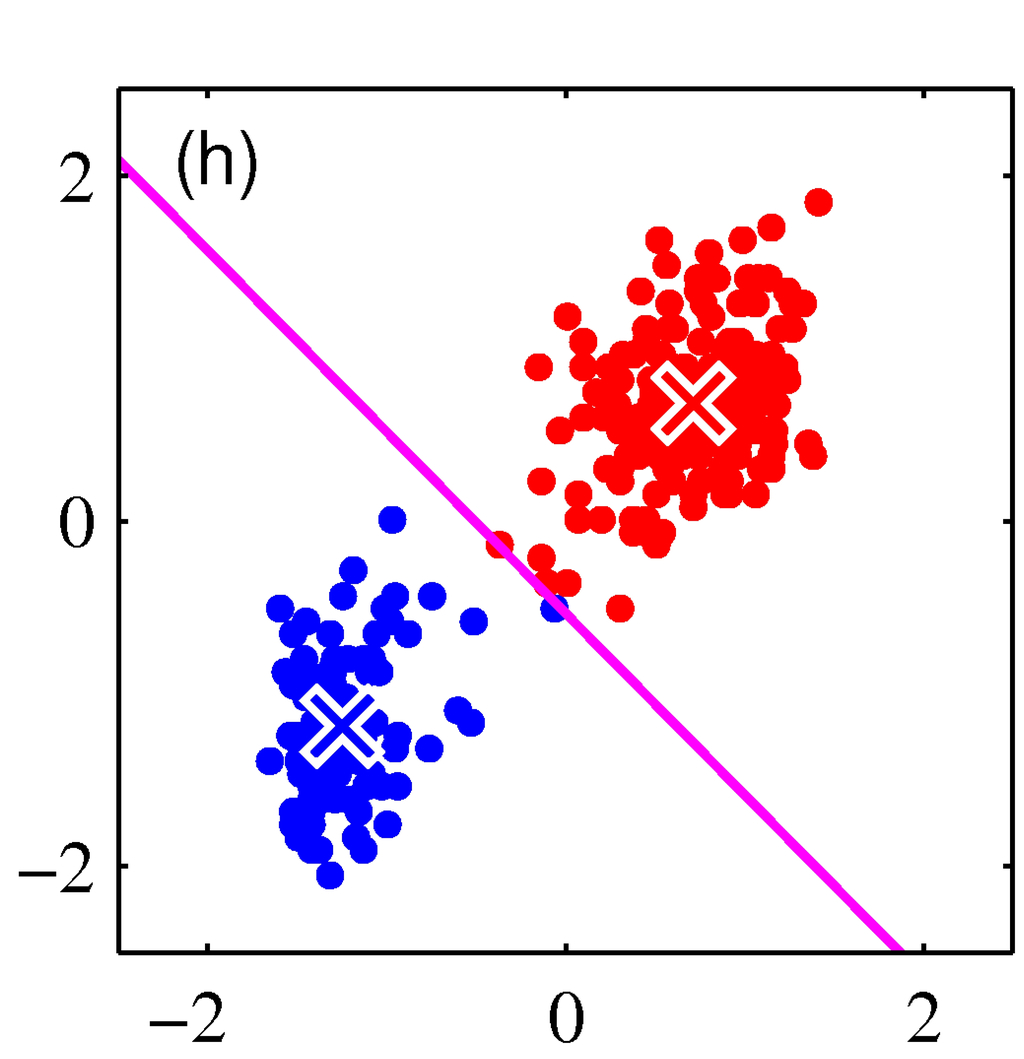
\includegraphics[width=0.65\textwidth]{fig/lec725.jpg}
	\end{center}
\end{frame}
% 26
\begin{frame}[c]
	\frametitle{K-means illustration}
	\begin{center}
		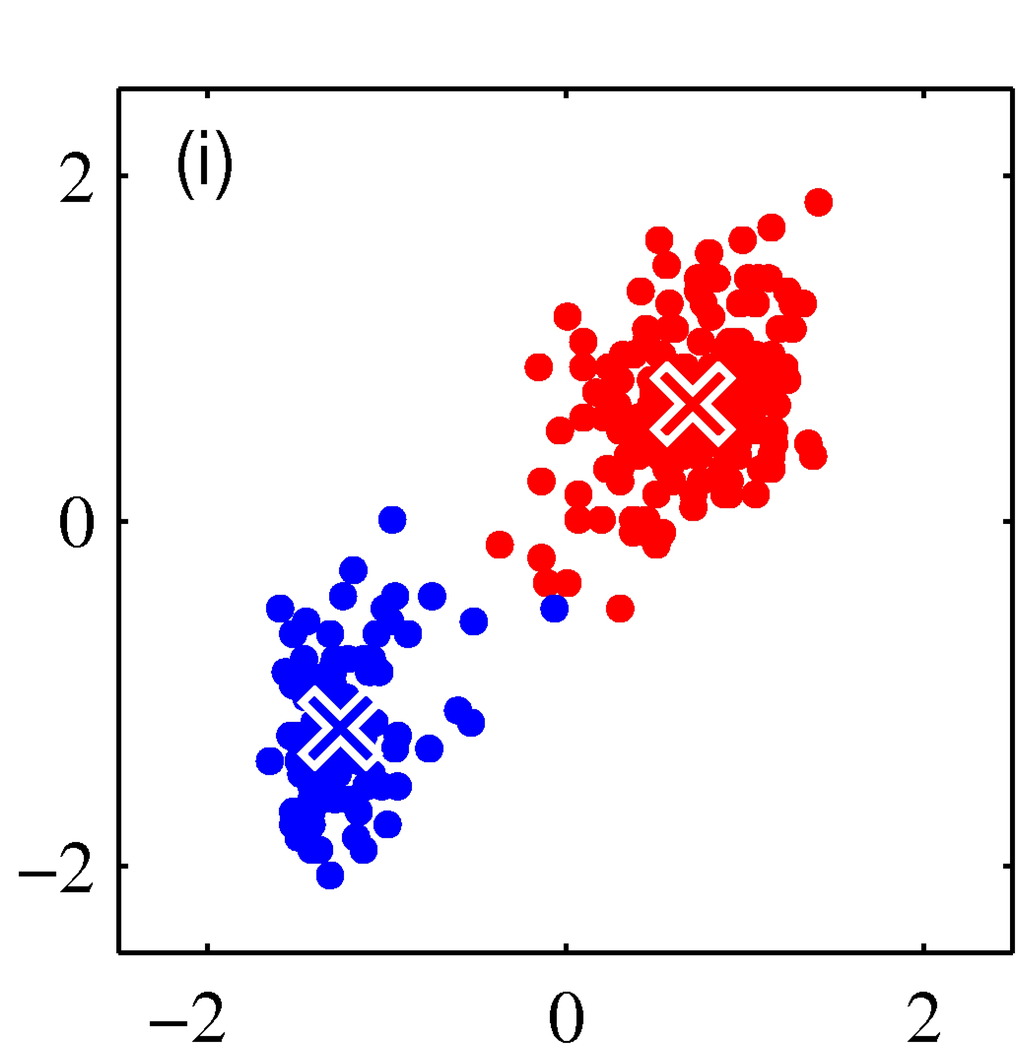
\includegraphics[width=0.65\textwidth]{fig/lec726.jpg}
	\end{center}
\end{frame}
% 27
\begin{frame}[c]
	\frametitle{K-means cost function}
	\begin{center}
		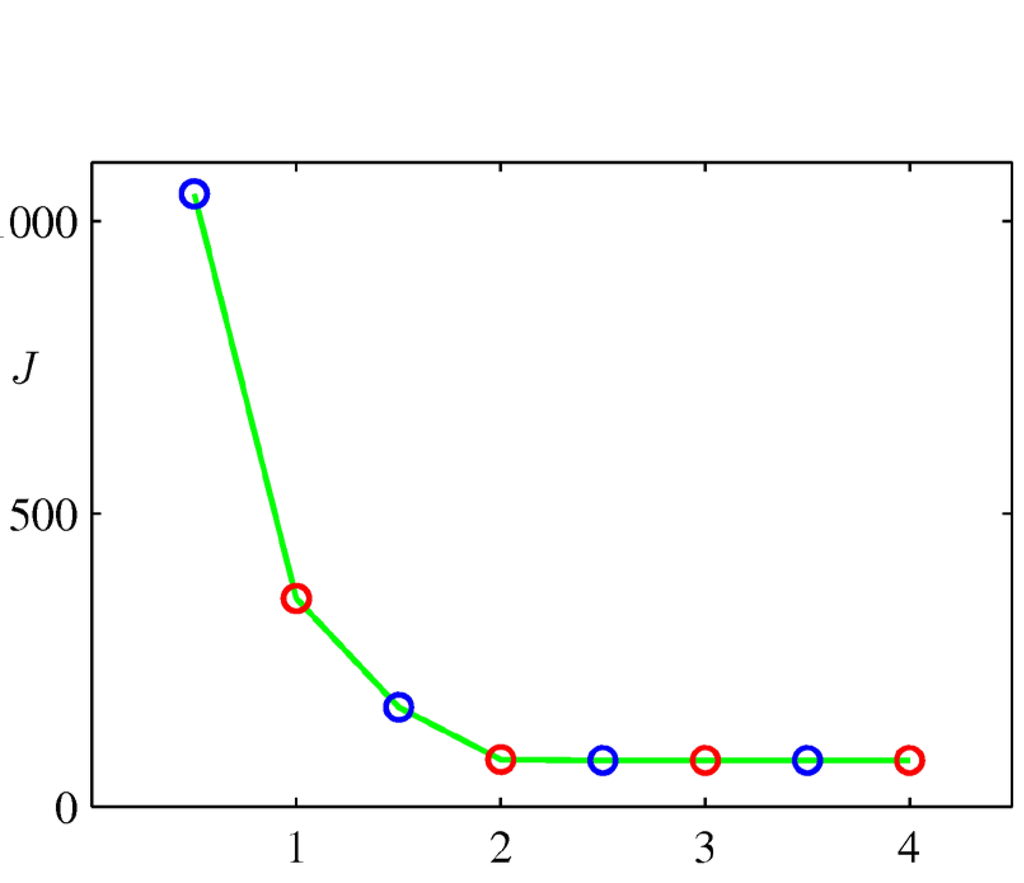
\includegraphics[width=0.65\textwidth]{fig/lec727.jpg}
	\end{center}
\end{frame}

% 28
\begin{frame}[c]
	\frametitle{K-means algorithm remarks}
	\begin{itemize}
		\item The K-means algorithm always converges, but only to a local minimum
	\end{itemize}
\end{frame}


% 29
\begin{frame}[c]
	\frametitle{2. How to determine the Gaussian widths?}
	\begin{itemize}
		\item Once cluster centers are determined, the variance within each cluster can be set to
		      \[
			      \sigma_j^2=\frac{1}{C_j}\sum_{i\in C_j}||\mathbf{u}_j-\mathbf{x}_i||^2
		      \]
		      \begin{itemize}
			      \item {\bf Remark:} to simplify the RBF net design, all clusters can assume the same Gaussian width:
			            \[
				            \sigma=\frac{d_{\max}}{\sqrt{2K}}
			            \]
			            where $d_{\max}$ is the maximum distance between the $K$ cluster centers
		      \end{itemize}
	\end{itemize}
\end{frame}

% 30
\begin{frame}[c]
	\frametitle{3. How do we determine the weights $w_j$?}
	\begin{itemize}
		\item With the hidden layer decided, weight training can be treated as a linear regression problem
		      \[
			      \mPhi \mathbf{w}=\mathbf{d}
		      \]
		\item Can solve using the LMS algorithm
		\item The textbook discusses recursive least squares (RLS) solutions
		\item Can also solve in one shot using the pseudo-inverse
		      \[
			      \mathbf{w}=\mPhi^+\mathbf{d}=(\mPhi^T\mPhi)^{-1}\mPhi^T\mathbf{d}
		      \]
		\item Note that a bias term needs to be included in ${\mPhi}$
	\end{itemize}
\end{frame}



% 31
\begin{frame}[c]
	\frametitle{4. How do we select the number of bases?}
	\begin{itemize}
		\item The same problem as that of selecting the size of an MLP for classification
		\item The short answer: (cross-)validation
		\item The long answer: by balancing bias and variance
	\end{itemize}
\end{frame}



% 32
\begin{frame}[c]
	\frametitle{Bias and variance}
	\begin{itemize}
		\item Bias: training error
		      \begin{itemize}
			      \item Difference between desired output and actual output for a particular training sample
		      \end{itemize}
		\item Variance: generalization error
		      \begin{itemize}
			      \item  difference between the learned function from a particular training sample and the function derived from all training samples
		      \end{itemize}
		\item Two extreme cases: zero bias and zero variance
		\item A good-sized model is one where both bias and variance are low
	\end{itemize}
\end{frame}


% 33
\begin{frame}[c]
	\frametitle{RBF net training summary}
	\begin{itemize}
		\item To train
		      \begin{enumerate}
			      \item Choose the Gaussian centers using K-means, etc.
			      \item Determine the Gaussian widths as the variance of each cluster, or using $d_{\max}$
			      \item Determine the weights $w_j$ using linear regression
		      \end{enumerate}
		\item Select the number of bases using (cross-)validation
	\end{itemize}
\end{frame}


% 34
\begin{frame}[c]
	\frametitle{RBF net illustration}
	\begin{center}
		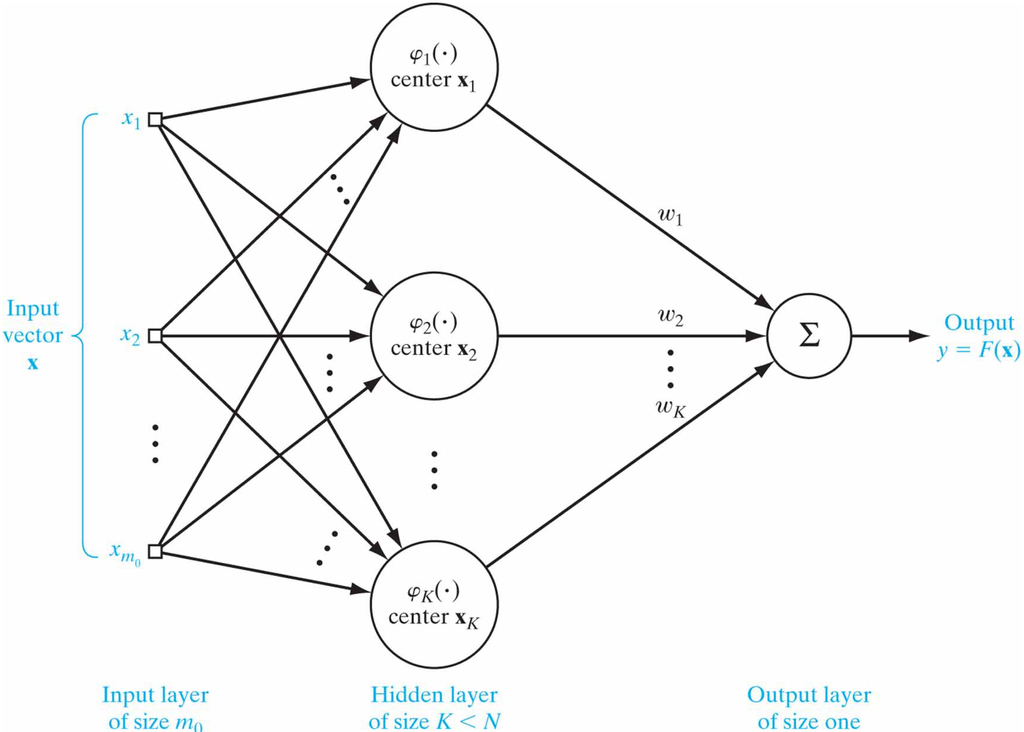
\includegraphics[width=0.99\linewidth]{fig/lec734.jpg}
	\end{center}
\end{frame}



% 35
\begin{frame}[c]
	\frametitle{Comparison between RBF net and MLP}
	\begin{itemize}
		\item For RBF nets, bases are local, while for MLP, ``bases'' are global
		\item Generally, more bases are needed for an RBF net than hidden units for an MLP
		\item Training is more efficient for RBF nets
	\end{itemize}
\end{frame}

% 36
\begin{frame}[t]
	\frametitle{XOR problem, again}
	\begin{columns}
		\column{.5\textwidth}

		\begin{itemize}
			\item RBF nets can also be applied to pattern classification problems
			      \begin{itemize}
				      \item XOR problem revisited
			      \end{itemize}
		\end{itemize}
		\column{.5\textwidth}
		\begin{center}
			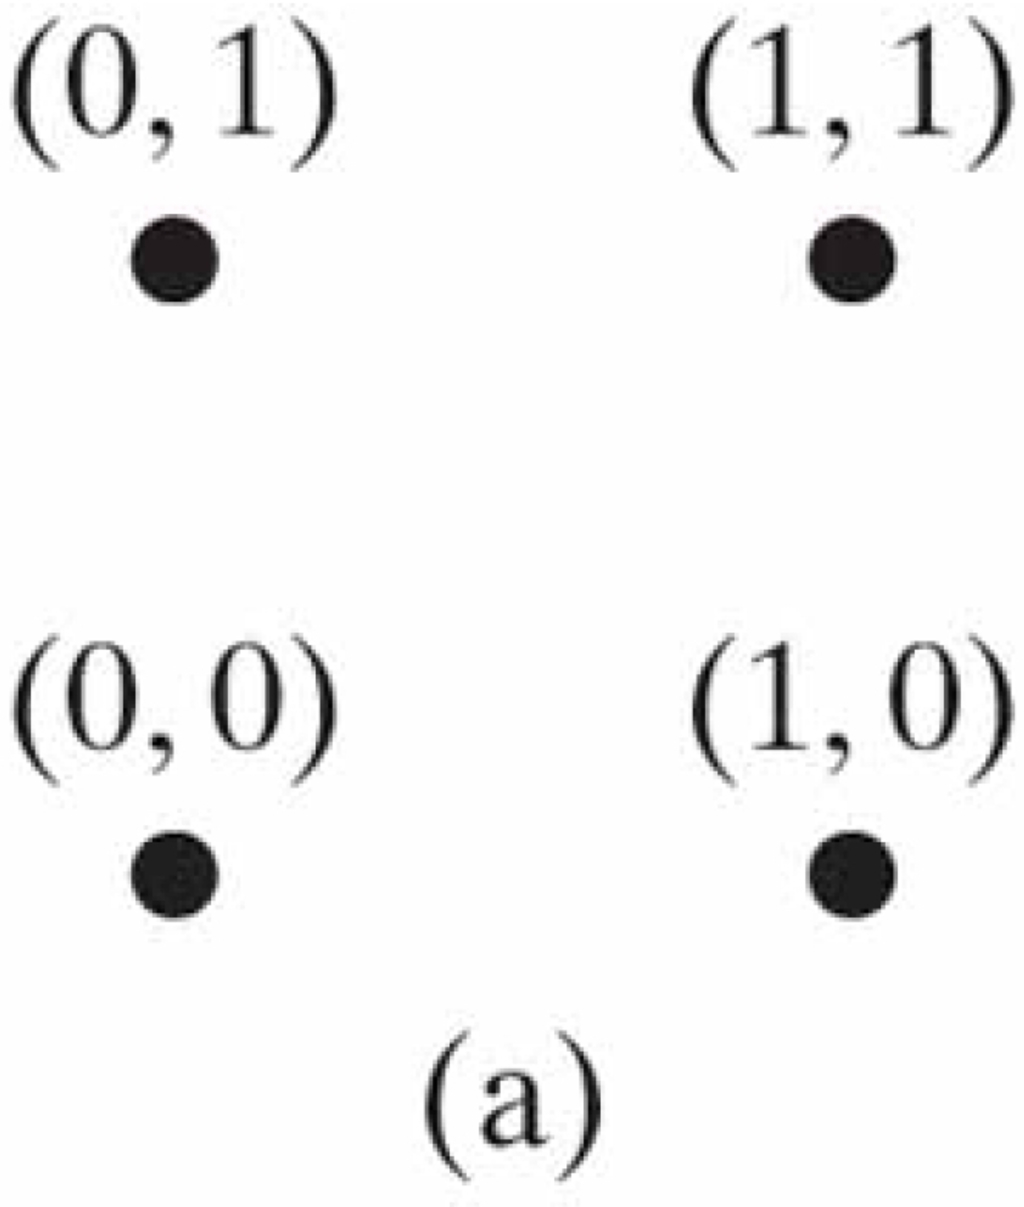
\includegraphics[width=0.3\linewidth]{fig/lec736.jpg}
		\end{center}
		Let

		$\phi_1(x)=\exp (-||x-t_1||)^2$

		$\phi_2(x)=\exp (-||x-t_2||)^2$

		where
		\[\begin{array}{c}
				t_1=[1,1]^T \\
				t_2=[0,0]^T
			\end{array}\]
	\end{columns}
\end{frame}


% 37
\begin{frame}[c]
	\frametitle{XOR problem (cont.)}
	\begin{center}
		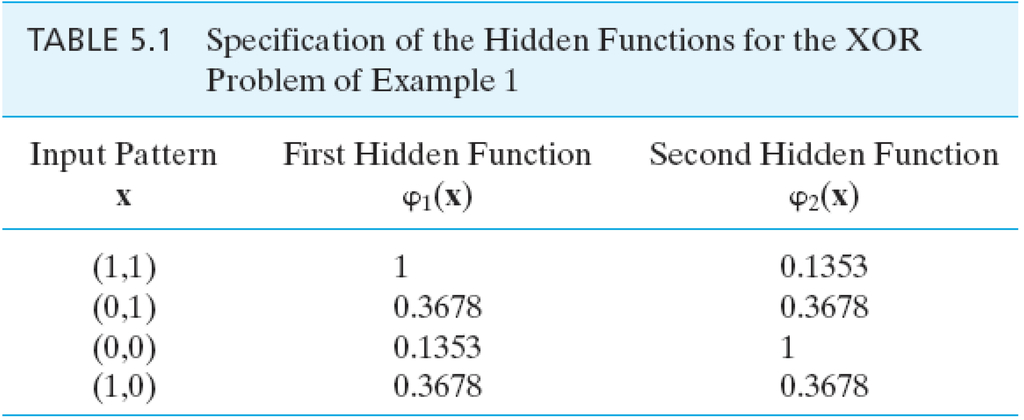
\includegraphics[width=0.95\linewidth]{fig/lec737.jpg}
	\end{center}
\end{frame}


% 38
\begin{frame}
	\frametitle{XOR problem, again}
	\begin{columns}
		\column{.5\textwidth}
		\begin{itemize}
			\item RBF nets can also be applied to pattern classification problems
			      \begin{itemize}
				      \item XOR problem revisited
			      \end{itemize}
		\end{itemize}
		\column{.5\textwidth}
		\begin{center}\hspace*{-5mm}
			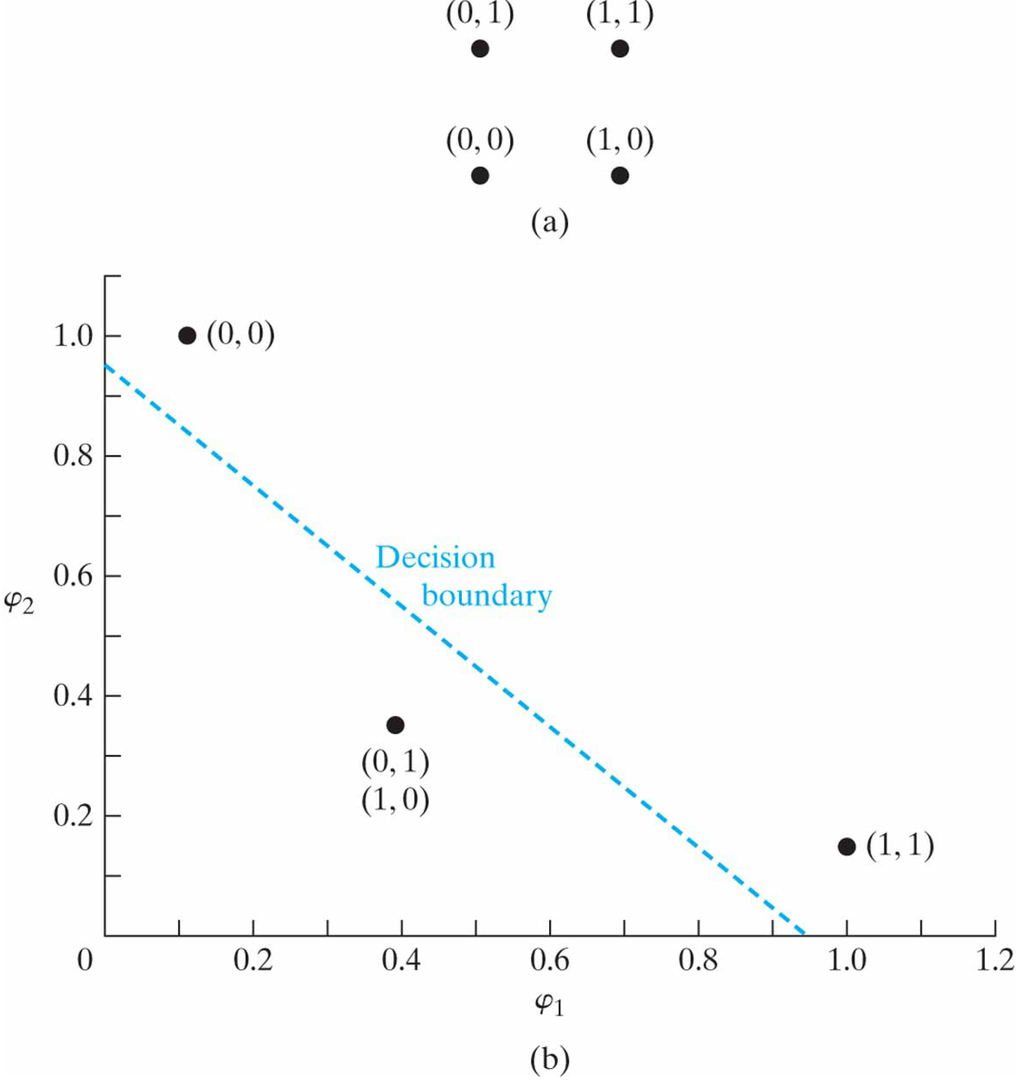
\includegraphics[width=1.15\linewidth]{fig/lec738.jpg}
		\end{center}
	\end{columns}
\end{frame}


% 39
\begin{frame}
	\frametitle{RBF net on double moon data, $d=-5$}
	\begin{center}
		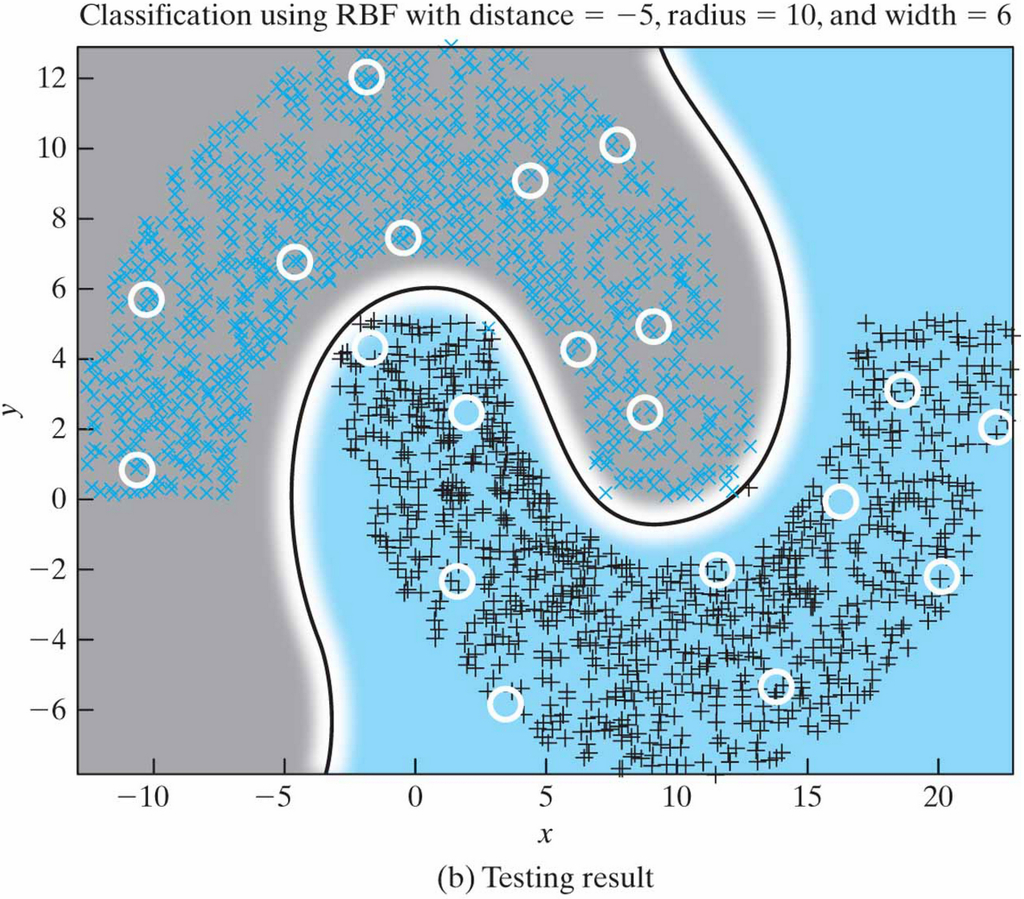
\includegraphics[width=0.8\linewidth]{fig/lec739.jpg}
	\end{center}
\end{frame}


% 40
\begin{frame}
	\frametitle{RBF net on double moon data, $d=-5$}
	\begin{center}
		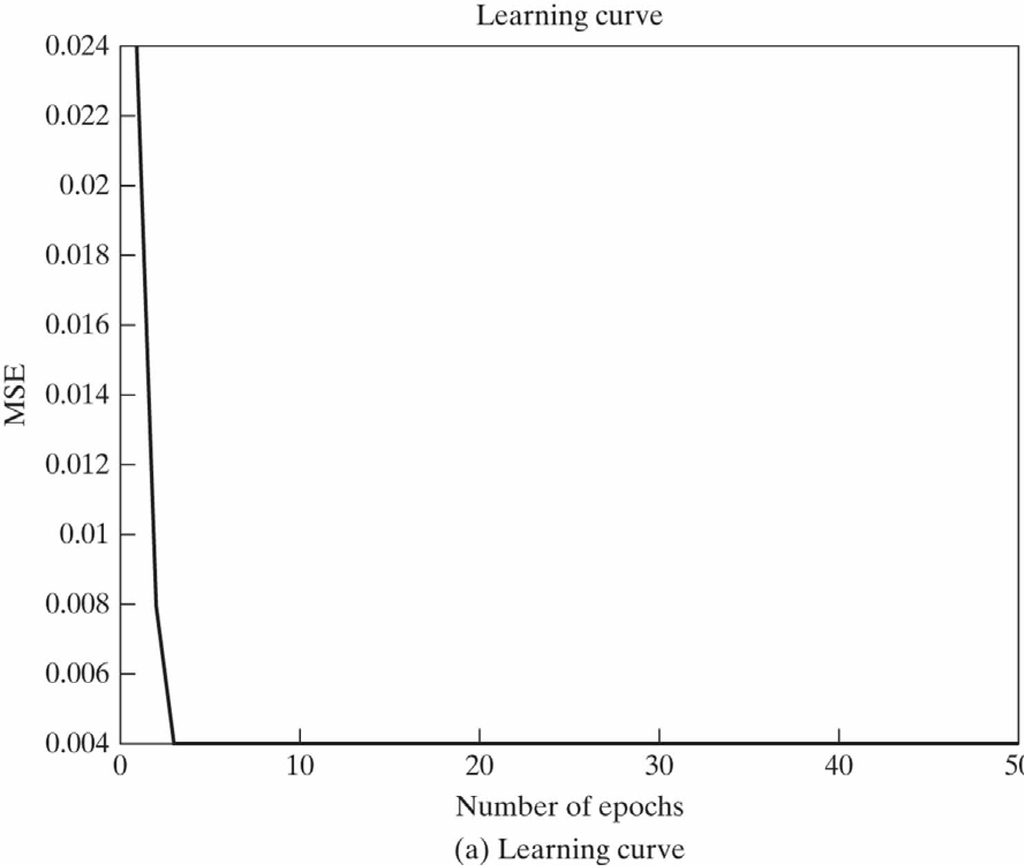
\includegraphics[width=0.8\linewidth]{fig/lec740.jpg}
	\end{center}
\end{frame}

% 41
\begin{frame}
	\frametitle{RBF net on double moon data, $d=-6$}
	\begin{center}
		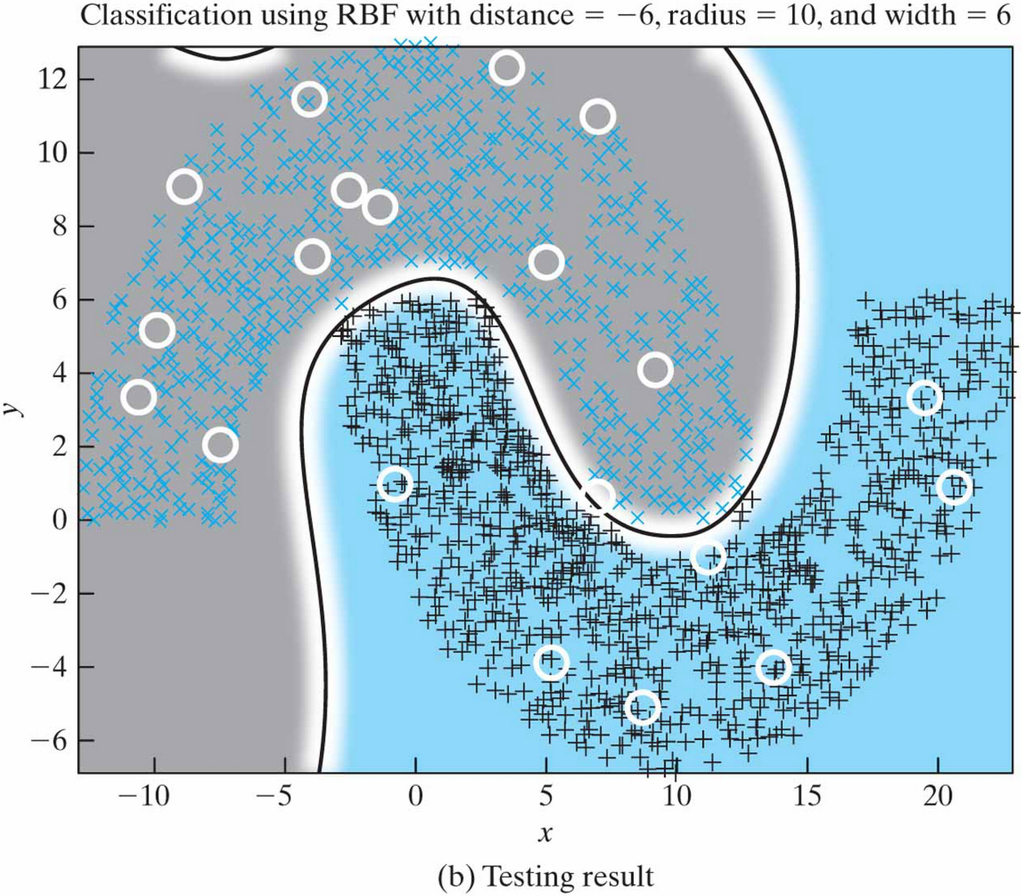
\includegraphics[width=0.8\linewidth]{fig/lec741.jpg}
	\end{center}
\end{frame}

% 42
\begin{frame}
	\frametitle{RBF net on double moon data, $d=-6$}
	\begin{center}
		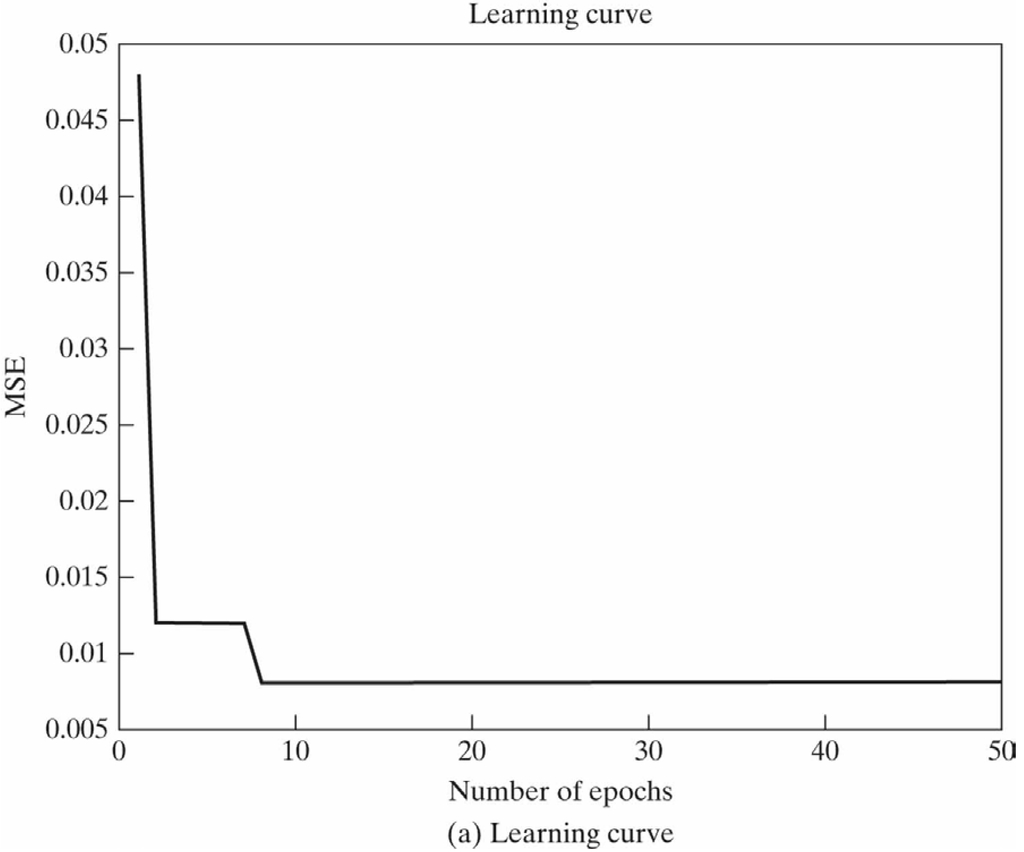
\includegraphics[width=0.8\linewidth]{fig/lec742.jpg}
	\end{center}
\end{frame}






\begin{frame}
	\begin{center}
		\chuhao Thank you! %\fontspec{LHANDW.TTF}
	\end{center}
\end{frame}
\end{document}
